\documentclass[tikz]{standalone}
\usepackage{tikz}
\usetikzlibrary{positioning}

\begin{document}

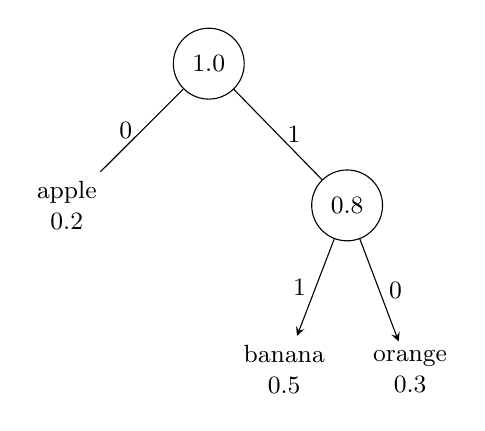
\begin{tikzpicture}[%
    >=stealth,
    level distance=18mm,
    sibling distance=26mm,
    every node/.style={font=\small}
]

% root = 1.0
\node[circle, draw, minimum size=9mm] (root) {$1.0$}
    child[left] {
        % apple leaf
        node[align=center] (apple) {apple\\$0.2$}
        edge from parent node[midway,  left] {0}
    }
    child[right] {
        % internal node for orange + banana
        node[circle, draw, minimum size=9mm] (node2) {$0.8$}
        edge from parent node[midway,  right] {1}
    };

% children of node2
\node[align=center, below=12.7mm of node2, xshift=8mm] (orange)
    {orange\\$0.3$};

\node[align=center, below=12mm of node2, xshift=-8mm] (banana)
    {banana\\$0.5$};

% edges from node2 to leaves manually
\draw[->] (node2) -- (orange) node[midway,right ] {0};
\draw[->] (node2) -- (banana) node[midway, left] {1};

\end{tikzpicture}

\end{document}